\documentclass[a4paper,12pt]{book}

\setlength{\headheight}{1.1\baselineskip}
 
\usepackage[utf8]{inputenc}
\usepackage[spanish]{babel}

\usepackage{geometry}
\usepackage[sc]{mathpazo}

\usepackage{mathtools}
\usepackage{amssymb}

\usepackage[usenames,dvipsnames]{color} 
\usepackage{hyperref}
\usepackage{alltt}

% Para footer con páginas
\usepackage{scrpage2}
\usepackage{lastpage}

% Para insertar imágenes y ubicarlas
\usepackage{graphicx}
\usepackage{placeins}

% Para insertar código
\usepackage{xcolor}
\usepackage{listings}

\usepackage[T1]{fontenc} %%%key to get copy and paste for the code!

\usepackage{amssymb,amsmath}

% Source Code
\usepackage{color}
\usepackage{textcomp}
\usepackage{listings}
\usepackage{amsfonts}
\usepackage{courier}

\definecolor{source}{gray}{0.9}

% my comment style
\newcommand{\myCommentStyle}[1]{{\ttfamily\footnotesize\color{gray!100!white} #1}}

% my string style
\newcommand{\myStringStyle}[1]{{\ttfamily\footnotesize\color{violet!100!black} #1}}

% my symbol style
\newcommand{\mySymbolStyle}[1]{{\ttfamily\footnotesize\color{violet!100!black} #1}}

% my keyword style
\newcommand{\myKeywordStyle}[1]{{\ttfamily\footnotesize\color{green!70!black} #1}}

% my global style
\newcommand{\myGlobalStyle}[1]{{\ttfamily\footnotesize\color{blue!100!black} #1}}

% my number style
\newcommand{\myNumberStyle}[1]{{\ttfamily\footnotesize\color{brown!100!black} #1}}

\lstset{
language={},
% characters
tabsize=3,
escapechar={!},
keepspaces=true,
breaklines=true,
alsoletter={\#},
literate={\$}{{{\$}}}1,
breakautoindent=true,
columns=fullflexible,
showstringspaces=false,
% background
frame=single,
aboveskip=1em, % automatic space before
framerule=0pt,
basicstyle=\ttfamily\footnotesize\color{black},
keywordstyle=\myKeywordStyle,% keyword style
commentstyle=\myCommentStyle,% comment style
frame=single,%
backgroundcolor=\color{source},
% numbering
stepnumber=1,
numbersep=10pt,
numberstyle=\tiny,
numberfirstline=true,
% caption
captionpos=b,
% formatting (html)
moredelim=[is][\bfseries]{<b>}{</b>},
moredelim=[is][\textit]{<i>}{</i>},
moredelim=[is][\underbar]{<u>}{</u>},
moredelim=[is][\color{red}\uwave]{<wave>}{</wave>},
moredelim=[is][\color{red}\sout]{<del>}{</del>},
moredelim=[is][\color{blue}\underbar]{<ins>}{</ins>},
% smalltalk stuff
morecomment=[s][\myCommentStyle]{"}{"},
%    morecomment=[s][\myvs]{|}{|},
morestring=[b][\myStringStyle]',
moredelim=[is][]{<sel>}{</sel>},
moredelim=[is][]{<rcv>}{</rcv>},
moredelim=[is][\itshape]{<symb>}{</symb>},
moredelim=[is][\scshape]{<class>}{</class>},
morekeywords={true,false,nil,self,super,thisContext},
identifierstyle=\idstyle,
}

\makeatletter
\newcommand*\idstyle[1]{%
\expandafter\id@style\the\lst@token{#1}\relax%
}
\def\id@style#1#2\relax{%
\ifnum\pdfstrcmp{#1}{\#}=0%
% this is a symbol
\mySymbolStyle{\the\lst@token}%
\else%
\edef\tempa{\uccode`#1}%
\edef\tempb{`#1}%
\ifnum\tempa=\tempb%
% this is a global
\myGlobalStyle{\the\lst@token}%
\else%
\the\lst@token%
\fi%
\fi%
}
\makeatother


%\newcommand{\ct}{\lstinline[backgroundcolor=\color{white}]}
%\newcommand{\needlines}[1]{\Needspace{#1\baselineskip}}
\newcommand{\lct}{\texttt}

\lstnewenvironment{code}{%
    \lstset{%
    % frame=lines,
    frame=single,
    framerule=0pt,
    mathescape=false
    }%
    \noindent%
    \minipage{\linewidth}%
}{%
    \endminipage%
}%


\lstnewenvironment{codeWithLineNumbers}{%
    \lstset{%
    % frame=lines,
    frame=single,
    framerule=0pt,
    mathescape=false,
    numbers=left
    }%
    \noindent%
    \minipage{\linewidth}%
}{%
    \endminipage%
}%

%For simple inlined code
\newcommand{\ct}{\texttt}

%utiles e.g., i.e., c.f.
\usepackage{xspace}
\newcommand{\eg}{\emph{e.g.,}\xspace}
\newcommand{\ie}{\emph{i.e.,}\xspace}
\newcommand{\cf}{\emph{c.f.}\xspace}

%For comments
\usepackage{ifthen}
\newboolean{showcomments}
\setboolean{showcomments}{true}
\ifthenelse{\boolean{showcomments}}
  {\newcommand{\bnote}[2]{
	\fbox{\bfseries\sffamily\scriptsize#1}
    {\sf\small$\blacktriangleright$\textit{#2}$\blacktriangleleft$}
    % \marginpar{\fbox{\bfseries\sffamily#1}}
   }
   \newcommand{\cvsversion}{\emph{\scriptsize$-$Id: macros.tex,v 1.1.1.1 2007/02/28 13:43:36 bergel Exp $-$}}
	\newcommand{\del}[1]{\bnote{Remove}{\textcolor{gray} #1}}
  }
  {\newcommand{\bnote}[2]{}
   \newcommand{\cvsversion}{}
	\newcommand{\del}[1]{}
  } 

\newcommand{\gp}[1]{\bnote{Guille}{#1}}
\newcommand{\fd}[1]{\bnote{Fer}{#1}}

\newtheorem{definition}{Definición}

\newenvironment{codeNonSmalltalk}
{\begin{alltt}\ttfamily}
{\end{alltt}\normalsize}

% Para insertar boxes
\usepackage[framemethod=TikZ]{mdframed}
\mdfdefinestyle{BoxFrame}{%
    linecolor=black,
    outerlinewidth=1pt,
    roundcorner=20pt,
    innertopmargin=\baselineskip,
    innerbottommargin=\baselineskip,
    innerrightmargin=20pt,
    innerleftmargin=20pt,
    backgroundcolor=gray!30!white}

\renewcommand{\labelitemi}{$\bullet$}
\renewcommand{\labelitemii}{$\cdot$}
\renewcommand{\labelitemiii}{$\diamond$}
\renewcommand{\labelitemiv}{$\ast$}  

\ifoot[]{}
\ofoot[]

\pagestyle{scrplain}

\vspace{0.1in}

\definecolor{dkgreen}{rgb}{0,0.6,0}
\definecolor{gray}{rgb}{0.5,0.5,0.5}
\definecolor{mauve}{rgb}{0.58,0,0.82}

\begin{document}

\chapter{Colecciones}
por Fernando Dodino
\\
\\
Las colecciones son un concepto importante y poderoso al diseñar con objetos. En este capítulo veremos cómo
se modela el conocimiento de un conjunto de referencias de un objeto y su utilización para resolver un problema
concreto.
\\
\\

\tableofcontents

\section{Introducción}

\subsection{¿Qué es una colección?}
La colección nos permite representar un conjunto de objetos relacionados: los jugadores de un equipo de fútbol, 
un cardumen de peces, las cosas que un héroe guarda en su mochila, un ejército, son ejemplos de este
tipo de abstracciones.\\
\\
Otra definición posible es que una colección nos sirve para modelar una relación 1 a N:\\
\begin{itemize}
\item Una factura tiene muchas líneas con productos
\item Un escritor publicó varios libros
\item Una fiesta tiene muchos invitados
\item Un héroe tiene que cumplir varias misiones
\end{itemize}

A primera vista una colección es un conjunto de objetos. Si la vemos con más precisión nos damos cuenta que es más
preciso pensarla como un conjunto de referencias: los elementos no están adentro de la colección, sino que la
colección los conoce. 
\\
\\
\begin{figure}
    \centering
    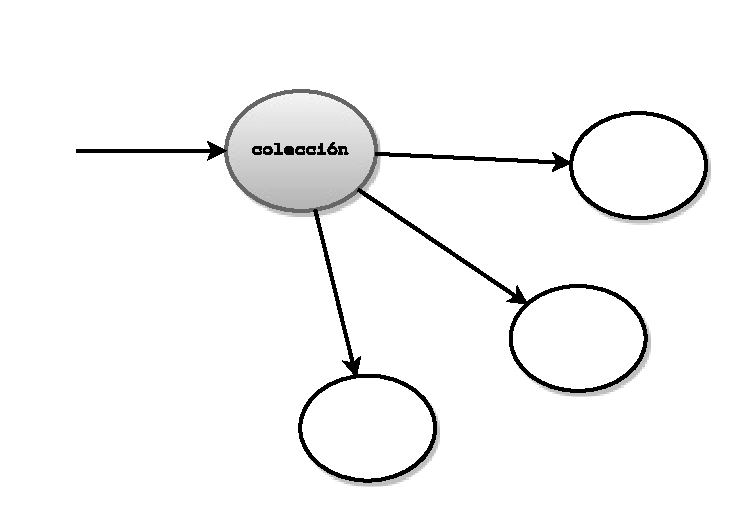
\includegraphics[width=0.8\textwidth]{images/01_GraficoInicial_Colecciones.pdf}
    \caption{La colección es un conjunto de referencias a otros objetos}
\end{figure}
\\
\subsection{Representación de colecciones}
Podemos graficar la relación dinámica entre un equipo de fútbol y los jugadores que lo integran mediante un diagrama
de objetos. Este es un diagrama con características \textit{dinámicas}, porque muestra el estado 
de los objetos en un momento determinado.
\\
\begin{figure}[h!]
    \centering
    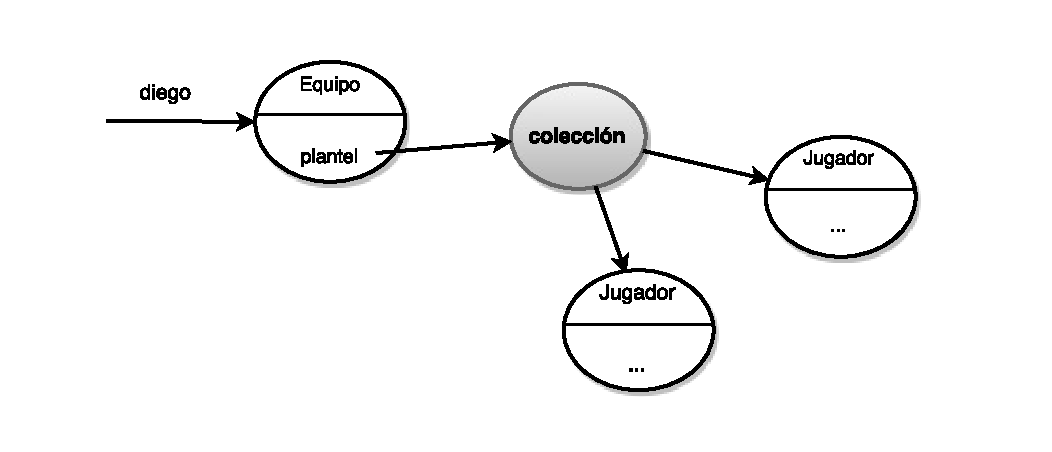
\includegraphics[width=1.1\textwidth]{images/02_Diagrama_Objetos_Equipo.pdf}
    \caption{El plantel de jugadores de un equipo como una colección de objetos}
\end{figure}
\FloatBarrier
También podemos generar un diagrama de clases en UML de la misma relación:
\begin{figure}[h!]
    \centering	
    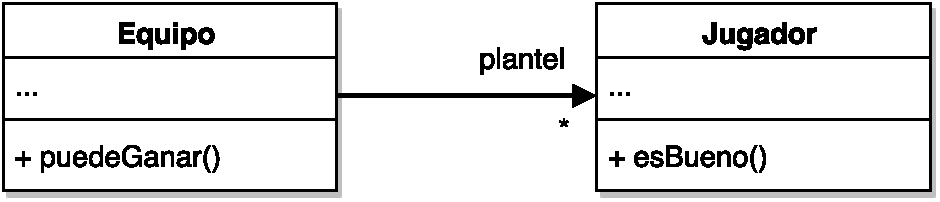
\includegraphics[width=0.9\textwidth]{images/03_Diagrama_Clases_Equipo.pdf}
    \caption{El plantel de jugadores, visto al nivel de clases}
\end{figure}
\FloatBarrier
Este es un diagrama con características \textit{estáticas}, porque no depende de un caso particular
sino que muestra las relaciones entre las clases.\\
\\
¿Qué es lo que cuenta el diagrama? Que un equipo \textbf{tiene} jugadores, el conector marca una relación
de \textbf{asociación}: hay un atributo plantel en la clase Equipo (el nombre del atributo se marca en uno
de los extremos de la asociación). El asterisco (*) muestra la multiplicidad: un equipo tiene muchos jugadores.
La dirección marca qué objeto conoce a los otros: como la flecha va de Equipo a Jugador sabemos que cada equipo
tiene n jugadores, no conocemos qué características tiene la relación de Jugador a Equipo, pero se pueden dar
dos opciones:
\begin{itemize}
\item un jugador pertenece a un solo equipo, en ese caso la relación Equipo-Jugador es de \textbf{uno a muchos}
\item un jugador participa en una relación con varios equipos (por ejemplo, porque nos interesa saber
en qué equipos jugó). En ese caso la relación es de \textbf{muchos a muchos}
\end{itemize}

\section{Interfaz de una colección}
Supongamos que tenemos un álbum de fotos, otra representación posible de una colección de objetos.
¿Qué podemos hacer con esas fotografías?
\\
\begin{itemize}
\item Mirarlas, ``recorrerlas'': iterar una colección
\item Averiguar cuántas fotos hay: saber su longitud
\item Saber si está una determinada foto en el álbum: saber si un elemento pertenece a la colección
\item Pegar una foto nueva: agregar un elemento a la colección
\item Regalar una foto a alguien: eliminar un elemento de la colección
\item Buscar qué fotos son de Ushuaia: filtrar/seleccionar elementos de una colección
\item Anotar las personas que salieron en mis fotos: transformar los elementos de una colección
\item Saber si hay alguna foto de Navidad: determinar si alguno/todos los elementos satisfacen 
un criterio
\end{itemize}
En el último requerimiento aparece también la idea de conjunto vacío. 
En general podemos asociar la noción matemática de conjunto a la colección, aunque sabemos que el conjunto
matemático no tiene orden, ni se ``recorre'', mientras que en la colección eso depende de la intención que
nosotros tengamos, como veremos más adelante.
\\
\section{Un ejemplo concreto: Misiones de un héroe}
En ciertos casilleros el héroe puede encontrar misiones y nuevos objetivos. Por ejemplo, un mago puede
encargarle buscar un ítem mágico en una montaña lejana. Un anciano puede encargarle liberar a su hija de
los terribles trolls que habitan en la gruta de los sin nariz. Cada vez que un héroe tiene uno de estos
encuentros, él anota los datos de la misión en su diario personal. Cada vez que una misión es superada,
el héroe la marca como “cumplida”. Toda misión suma en el camino del héroe: las misiones tienen una
recompensa de oro, y de respeto.
\\
\\
¿Qué abstracciones surgen? El héroe ahora tiene una colección de misiones. En principio vamos a pensar en
dos tipos de misiones: 1) buscar un ítem mágico, 2) liberar a una doncella. Las misiones deben tener una
recompensa (más adelante podemos modelar unidades de oro o de respeto para ello), un solicitante y el estado,
que puede ser pendiente o cumplida. 
\\
\\
Además nos avisan que existen misiones difíciles, que son aquellas que tienen más de 2 meses de iniciada, 
y además
\begin{itemize}
 \item si la montaña donde está el ítem a buscar queda a más de 100 kms. o bien 
 \item si la doncella a liberar está custodiada por más de 4 trolls
\end{itemize}

\subsection{Generar el atributo colección}
Vamos a crear lo mínimo necesario para poder meternos de lleno en el ejemplo de las colecciones.
Ahora el héroe tendrá una colección de misiones:

\begin{code}
Object subclass: #Heroe
	instanceVariableNames: 'misiones ...'
\end{code}

También vamos a crear una misión posible: BuscarItemMagico, por el momento sin atributos, porque nos queremos
seguir concentrando en la interfaz y no en la implementación, es decir, qué me ofrece el objeto y no cómo lo
resuelve.

Para poder agregar una misión, vamos a definir un método explícito:

\begin{code}
#Heroe
agregarMision: unaMision
  misiones add: unaMision
\end{code}

\subsection{Primeras pruebas}
Abrimos un Workspace de trabajo o Playground y vamos a inicializar un juego de variables nuevo:

\begin{code}
diego := Heroe new
  agregarMision: (BuscarItemMagico new)
\end{code}

Al intentar enviar el mensaje agregarMision: recibimos el primer error, no existe la clase BuscarItemMagico,
entonces lo creamos:

\begin{figure}[h!]
    \centering	
    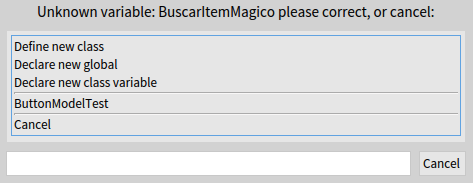
\includegraphics[width=0.8\textwidth]{images/16_crear_nueva_clase.png}
    \caption{Creando una clase a demanda}
\end{figure}
\FloatBarrier

Elegimos la opción ``Define new class'' sin preocuparnos todavía por los atributos

\begin{code}
Object subclass: #BuscarItemMagico
		instanceVariableNames: '' 
		classVariableNames: ''
		poolDictionaries: ''
		category: 'Kernel-Objects'
\end{code}

Una vez resuelta la creación de la clase, aparece un nuevo error, seleccionamos la opción Debug...

\begin{figure}[h!]
    \centering	
    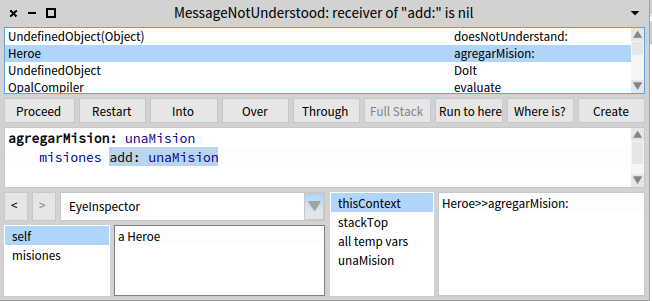
\includegraphics[width=0.7\textwidth]{images/11_error_agregarMision.png}
    \caption{La pantalla de \textit{debugging} muestra que el error ocurre al enviar el mensaje add: a misiones}
\end{figure}
\FloatBarrier

Esto se da porque la referencia a misiones quedó en nil. 

\begin{figure}[h!]
    \centering	
    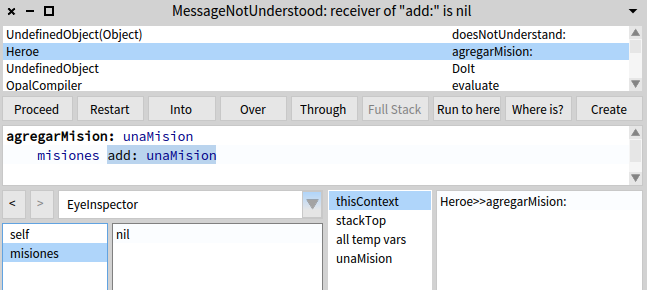
\includegraphics[width=1\textwidth]{images/12_error_debugging_2.png}
    \caption{misiones es una referencia a \textit{nil}, ¡falta inicializarla!}
\end{figure}
\FloatBarrier

Entonces debemos inicializar a diego cuando creemos el guerrero, esto lo podemos hacer manualmente o con la opción
Analyze \textgreater Generate initialize method

\begin{figure}[h!]
    \centering	
    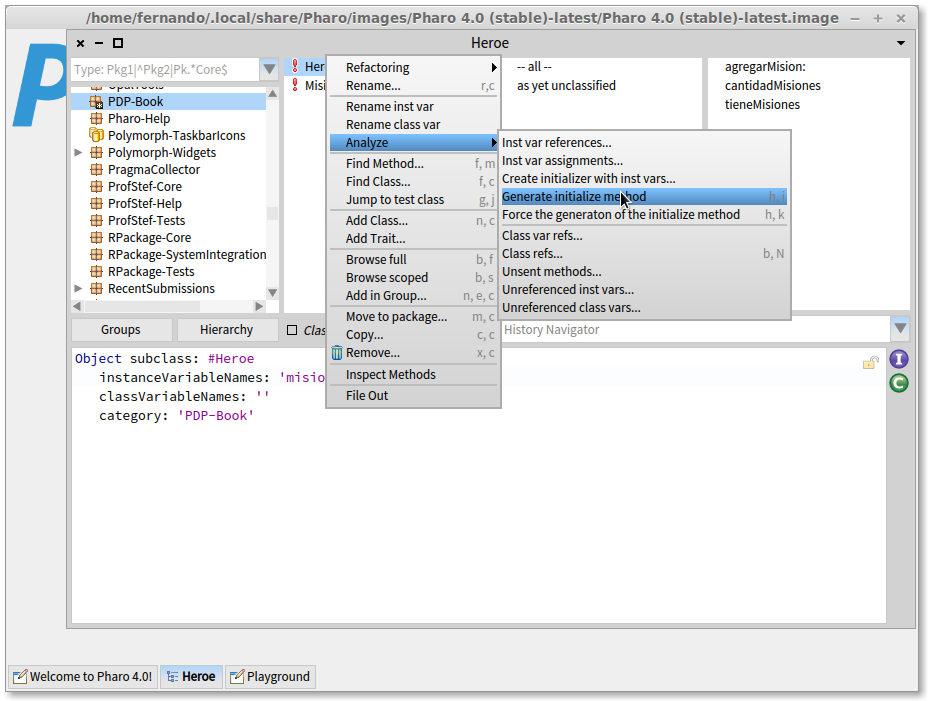
\includegraphics[width=0.9\textwidth]{images/13_generate_initialize.png}
    \caption{Generando un método initialize a través del IDE}
\end{figure}
\FloatBarrier

Comenzaremos usando un Set como colección, esto presupone que no nos importa el orden en el que almacenamos las
misiones y que no hay elementos duplicados: puede haber muchas liberaciones de doncellas, pero cada una 
representa una misión distinta. El Set es la implementación más equivalente al concepto matemático de conjunto
que presentamos anteriormente.
\\
\\
Ahora sí nuestro método nos queda

\begin{code}
#Heroe
initialize
	super initialize.
	misiones := Set new.
\end{code}


Al grabarlo volvemos al Playground y ejecutamos nuevamente el código mediante Do It

\begin{code}
diego := Heroe new
  agregarMision: (BuscarItemMagico new)
\end{code}


Vemos que el mensaje tuvo efecto inspeccionando la referencia diego: escribimos diego y luego Inspect It:

\begin{figure}[h!]
    \centering	
    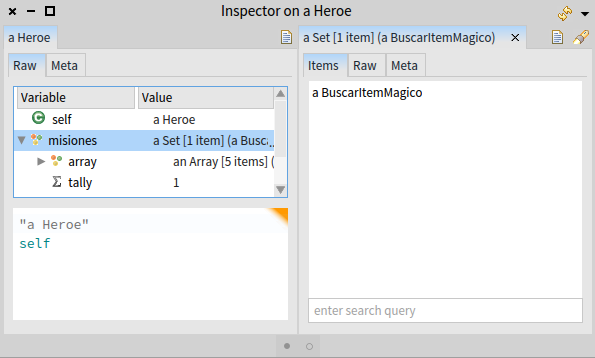
\includegraphics[width=0.9\textwidth]{images/14_coleccion_inicial.png}
    \caption{diego es un héroe y tiene una referencia en la colección misiones}
\end{figure}
\FloatBarrier


\subsection{Conocer el tamaño de una colección}
¿Cómo sabemos cuántas misiones tiene un héroe?

\begin{code}
#Heroe
cantidadMisiones
    ^misiones size
\end{code}
Y lo probamos, sabiendo que nos importa lo que va a devolver porque no es un método que tenga efecto, sino que
devuelve información, entonces elegimos la opción \textit{Print It}:

\begin{figure}[h!]
    \centering	
    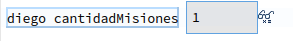
\includegraphics[width=0.6\textwidth]{images/15_diego_cantidadMisiones.png}
    \caption{diego tiene por el momento una sola misión}
\end{figure}
\FloatBarrier

\subsection{Saber si una colección tiene elementos}
Queremos saber si un héroe tiene misiones...

\begin{code}
#Heroe
// Opcion 1
tieneMisiones
    ^misiones notEmpty
\end{code}

    
\begin{code}
// Opcion 2
tieneMisiones
    ^misiones size > 0
\end{code}

Ambas opciones parecen similares, de todas maneras la primera opción es más \textit{expresiva}. En la segunda
opción hay una traducción implícita: size \textgreater  0.... ah, es si tiene elementos. Es un detalle, 
pero un detalle que implica tiempo que se pierde cada vez que vaya a leer la implementación de este método.
\\
\\
Lo probamos...

\begin{code}
diego tieneMisiones
\end{code}

\subsection{Subclases nuevas para Misión}
Creamos la clase Mision, con atributos solicitante, recompensa, fecha de inicio y fecha de cumplimiento. 
Para cada uno de ellos definiremos los accessors correspondientes, haciendo botón derecho sobre la clase
Mision > Refactoring > Inst Var Refactoring > Accessors 


\begin{figure}[h!]
    \centering
    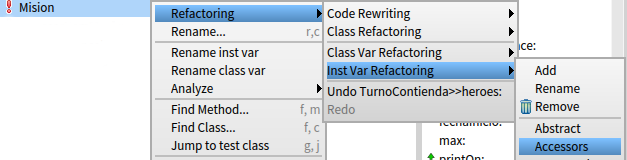
\includegraphics[width=0.9\textwidth]{images/10_accessors.png}
    \caption{El plantel de jugadores de un equipo como una colección de objetos}
\end{figure}

Dos subclases heredarán de Mision: 

\begin{itemize}
 \item BuscarItemMagico, necesitamos el atributo distanciaMontania
 \item LiberarDoncella, del cual necesitamos el atributo trollsSeguridad
\end{itemize}

Cambiaremos dinámicamente la superclase de BuscarItemMagico...

\begin{code}
Mision subclass: #BuscarItemMagico
	instanceVariableNames: 'distanciaMontania'
	classVariableNames: ''
	category: 'PDP-Book'
\end{code}

Damos ok al mensaje de advertencia y ahora tenemos a BuscarItemMagico como subclase de Mision.
\\
\\
Ahora definimos LiberarDoncella:

\begin{code}
Mision subclass: #LiberarDoncella
	instanceVariableNames: 'trollsSeguridad'
	classVariableNames: ''
	category: 'PDP-Book'
\end{code}

Una vez definidos los accessors, nos preguntamos: ¿qué comportamiento tiene una misión? Debe decirnos
si es difícil. Sabemos que esto depende de algo general (más de 2 meses de iniciada una misión) y se
especializa en cada subclase. Lo general... se codifica en la clase Misión:

\begin{code}
#Mision
esDificil
	^(self estaIniciadaHace: 60)
\end{code}

Claro, pero además debemos dejar que la misión delegue el comportamiento en cada implementación

\begin{code}
#Mision
esDificil
	^(self estaIniciadaHace: 60) & (self realmenteEsDificil)
\end{code}

Antes de resolver el método realmenteEsDificil, dejamos una posible implementación de estaIniciadaHace:

\begin{code}
#Mision
estaIniciadaHace: xDias
      ^(self estaAbierta) & ((Date new subtractDate: fechaInicio) > xDias)
      
estaAbierta
      ^fechaCumplimiento isNil       
\end{code}

Ahora sí el método realmenteEsDificil depende de este requerimiento:
\begin{itemize}
 \item si la montaña donde está el ítem a buscar queda a más de 100 kms. o bien 
 \item si la doncella a liberar está custodiada por más de 4 trolls
\end{itemize}

\begin{code}
#BuscarItemMagico
realmenteEsDificil      
  ^distanciaMontania > 100

#LiberarDoncella
realmenteEsDificil      
  ^trollsSeguridad > 4
\end{code}

Por motivos didácticos no vamos a explicar cómo se prueba la funcionalidad recientemente incorporada, pero
sabemos que este paso es fundamental para no tener inconvenientes con los pasos que vamos a hacer a continuación.

\subsection{Nuevas misiones para el héroe}
Vamos a asociar nuevas misiones a diego:

\begin{code}
diego := Heroe new
  agregarMision: (BuscarItemMagico new 
			distanciaMontania: 1000;
			solicitante: 'Mago de Oz';
			recompensa: 2000;
			fechaInicio: (Date newDay: 2 month: 2 year: 2004);
			yourself);
  agregarMision: (LiberarDoncella new 
			trollsSeguridad: 3;
			solicitante: 'Old man';
			recompensa: 10000;
			fechaInicio: (Date yesterday);
			yourself);
  agregarMision: (BuscarItemMagico new 
			distanciaMontania: 30;
			solicitante: 'Mago Cacarulo';
			recompensa: 500;
			fechaInicio: (Date yesterday);
			yourself);
  agregarMision: (LiberarDoncella new 
			trollsSeguridad: 7;
			solicitante: 'Old man';
			recompensa: 12000;
			fechaInicio: (Date yesterday);
			yourself).

\end{code}

\subsection{Filtrar elementos de una colección}
Queremos saber ahora qué misiones están abiertas.
\begin{itemize}
 \item El héroe conoce a sus misiones
 \item pero cada misión debe determinar si está abierta o no (es su \textbf{responsabilidad}). 
\end{itemize}

\begin{code}
#Heroe
misionesAbiertas
  ^misiones select: [ :mision | mision estaAbierta ] 
\end{code}

Redefinamos el printOn: de Misión para reflejar un poco más de información sobre el objeto:

\begin{code}
#Mision
printOn: aStream
   aStream nextPutAll: self descripcion;
		nextPutAll: ' para ';
		nextPutAll: self solicitante.
\end{code}

Redefinimos el método descripción para cada subclase:

\begin{code}
#BuscarItemMagico
descripcion
  ^'Buscar item magico'

#LiberarDoncella
descripcion
  ^'Liberar doncella'
\end{code}
  
Probamos entonces el nuevo método:

\begin{code}
diego misionesAbiertas
   a Set(Liberar doncella para Old man 
         Liberar doncella para Old man 
         Buscar item magico para Mago de Oz 
         Buscar item magico para Mago Cacarulo)
\end{code}

Claro, todas las misiones están abiertas. ¿Cómo cumplimos todas las misiones?
\\
\\
Tenemos el mensaje menos simpático para enseñar, el do:

\begin{code}
#Heroe
cumplirMisiones
  self misionesAbiertas do: [ :mision | mision cumplir ] 
  
#Mision
cumplir
  fechaCumplimiento := Date new
\end{code}

En el Playground le pedimos a diego que cumpla todas sus misiones pendientes:

\begin{code}
diego cumplirMisiones
\end{code}

Y ahora veamos si efectivamente el método tuvo efecto:

\begin{code}
diego misionesAbiertas
      a Set()
\end{code}

Antes de continuar es importante saber que estuvimos usando un concepto central en el uso de las colecciones...
\\

\section{Objetos bloque y declaratividad}
¿Por qué dijimos que el método do: es el menos simpático? Porque si bien ignoramos de qué manera se recorre la
colección tenemos la posibilidad de hacer algo con cada elemento de la colección, por ejemplo
\begin{itemize}
 \item ignorar determinados elementos
 \item o transformar los elementos de la colección
 \item o utilizar variables de diferente alcance: variables internas al bloque do:, variables locales en el mismo
 método, o variables globales, como las variables de instancia, o las de clase
\end{itemize}
A lo largo del libro intentaremos pensar nuestras soluciones utilizando bloques de más alto nivel, que aumenten
la \textbf{declaratividad}, esto es no pensar tanto en el algoritmo, o cómo se resuelve, sino en lo que nosotros
queremos lograr (el qué). Para eso utilizaremos objetos \textbf{closures} que modelan bloques de código 
(los que se encierran entre corchetes) y la rica interfaz de colecciones que provee Smalltalk.

¿Cómo se modela un bloque de código? Muy fácil:

\begin{code}
factorialDe5 := [ 5 factorial ].
\end{code}

Esto no ejecuta el factorial de 5, sino que crea un objeto que sabe calcularlo. Para evaluarlo efectivamente, 
debemos pedírselo:

\begin{code}
factorialDe5 value
    120
\end{code}

También podemos crear objetos bloque donde le pasemos parámetros:

\begin{code}
factorial := [ :numero | numero factorial ].
\end{code}

Pero ahora ya no podemos evaluarlo con value:

\begin{code}
factorial value
\end{code}

Esto nos muestra el mensaje de error:

\begin{figure}[h!]
    \centering	
    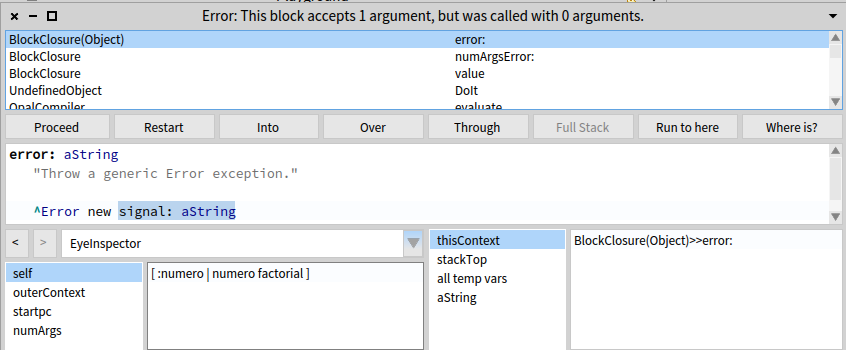
\includegraphics[width=0.9\textwidth]{images/17_error_bloque.png}
    \caption{El bloque espera un parámetro y no se lo pasamos}
\end{figure}
\FloatBarrier

Ahora si enviamos el valor, podemos calcular el factorial correspondiente:

\begin{code}
factorial value: 5
\end{code}

Tener un objeto bloque nos permite modelar, por ejemplo, un criterio de búsqueda ad-hoc:

\begin{code}
misionesConRecompensaMayorA: unValor
  | criterio |
  criterio := [ :mision | mision recompensa > unValor ].
  ^misiones select: criterio 
\end{code}

Esto nos permite probar:

\begin{code}
diego misionesConRecompensaMayorA: 2000
\end{code}

El criterio es un bloque que recibe un parámetro llamado mision (que es cualquier objeto que entienda el mensaje
recompensa) y devuelve un valor booleano. Lo podemos probar en un workspace:

\begin{code}
[ :mision | mision recompensa > 2000 ] value: (LiberarDoncella new recompensa: 5000)
\end{code}

Cuántos objetos intervienen:

\begin{itemize}
 \item un objeto bloque que espera un parámetro, y entiende el mensaje value:
 \item otro LiberarDoncella
\end{itemize}

Tener al bloque de código como abstracción me permite separar dos momentos: cuando creo al objeto y le digo lo
que tiene que hacer, y cuando efectivamente lo ejecuta (enviándole el mensaje value, value: o value:value: en
base a la cantidad de parámetros que tenga).

\section{Operaciones con y sin efecto}

Hay un detalle que puede pasar inadvertido para el lector pero que es importante remarcar, el mensaje select:
\textbf{no tiene efecto} sobre la colección. Esto implica que la colección original no modifica sus referencias,
entonces si necesitamos obtener las misiones difíciles el select: devuelve una nueva colección con los elementos
que cumplen ese criterio...

\begin{figure}[h!]
    \centering
    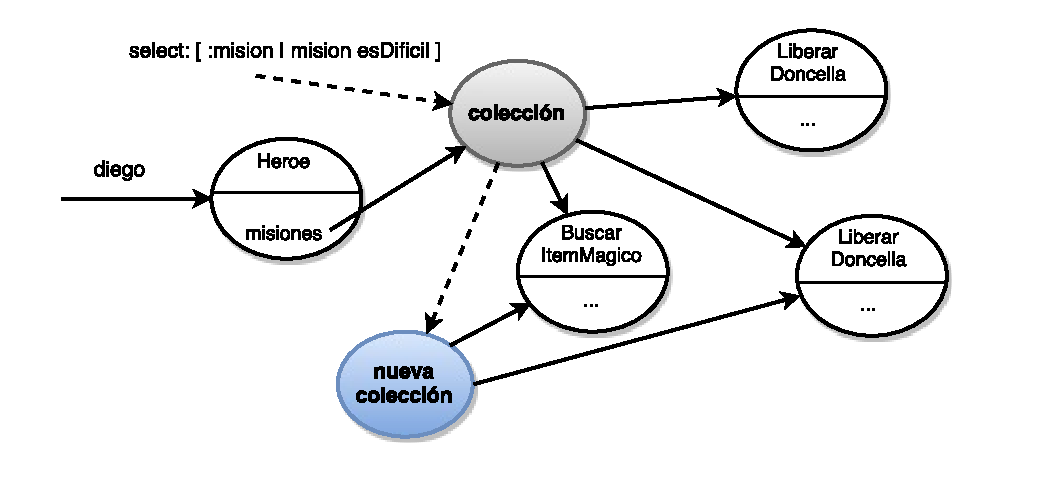
\includegraphics[width=1.1\textwidth]{images/20_select_sin_efecto.pdf}
    \caption{El select: no afecta a la colección original, devuelve una nueva colección}
\end{figure}


\section{Más sobre colecciones}

\subsection{Transformar los elementos de una colección}
Nos piden determinar quiénes son los solicitantes de las misiones de un héroe. Lo que sabemos es que cada
héroe tiene n misiones, y que cada misión tiene un solicitante, pero a su vez un solicitante puede pedir
varias misiones (la relación Solicitante-Misión es n a 1, o \textit{many-to-one}).
\\
\\
Entonces debemos
\begin{itemize}
 \item transformar cada misión en un solicitante
 \item y luego la lista de solicitantes debemos pasarla a un Set, para eliminar los duplicados.
\end{itemize}

Vemos la resolución:

\begin{code}
#Heroe
solicitantes
   ^(misiones collect: [ :mision | mision solicitante ]) asSet
\end{code}

Y lo probamos 

\begin{code}
diego solicitantes
   a Set('Mago Cacarulo' 'Old man' 'Mago de Oz')
\end{code}

Tampoco collect: es un método con efecto, genera una nueva colección:

\begin{figure}[h!]
    \centering
    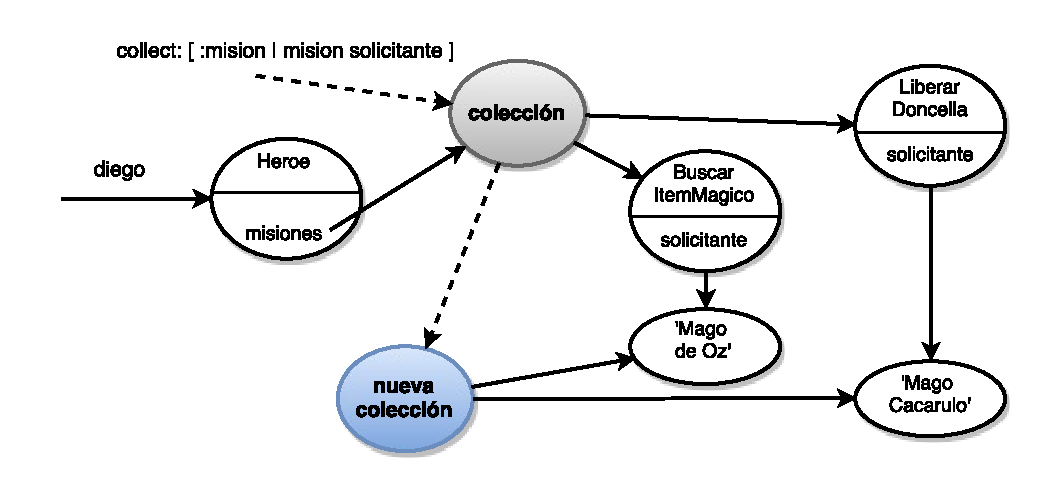
\includegraphics[width=1.1\textwidth]{images/21_Collect_sin_efecto.pdf}
    \caption{El collect: tampoco afecta a la colección original}
\end{figure}

\subsection{Encontrar un elemento que satisfaga una condición}
Si queremos encontrar la primera misión de un héroe cuya recompensa sea mayor a 500, 
podemos utilizar el mensaje detect:

\begin{code}
#Heroe
misionConBuenaRecompensa
    ^misiones detect: [ :mision | mision recompensa > 500 ]
\end{code}


\subsection{Totalizar valores de una colección}
Un nuevo requerimiento surge: hay que conocer la recompensa que obtendremos si cumplimos todas las misiones.
Esto implica sumar la recompensa de cada misión que esté pendiente. Tenemos varias opciones:
\\
\begin{itemize}
 \item iterar la colección mediante un do:, y utilizar una variable intermedia para acumular la recompensa
 preguntando previamente si la tarea se encuentra pendiente
 \item transformar las misiones pendientes en una colección de recompensas y sumarlas (aquí mediante do: o 
 bien enviando el mensaje sum. Para ver dónde está implementado pueden ubicarse en un workspace, escribir sum, 
 botón derecho y elegir Code search... \textgreater Implementors of it, o bien ver sus usos mediante botón derecho,
 Code search \textgreater Senders of it)
 \item y la tercera opción es sumarizar las tareas pendientes mediante el mensaje inject:into:
\end{itemize}

Veamos la solución primero:

\begin{code}
#Heroe
recompensaPendiente
   ^self misionesAbiertas 
         inject: 0 
	 into: [ :total :mision | total + mision recompensa ]
\end{code}

Lo probamos luego en un workspace, con la opción Print It, claro está:

\begin{code}
diego recompensaPendiente
  24500
\end{code}

El método inject:into: permite reducir la colección a la expresión deseada, es un método poderoso una vez que
nos acostumbramos a su sintaxis. Lo que necesita es

\begin{itemize}
 \item un valor inicial a inyectarse 
 \item un bloque de código que acepte dos argumentos y que devuelva el nuevo valor que se pasa a cada iteración siguiente
\end{itemize}

al final de la última iteración se devuelve el resultado final.
\\
\\
Veamos el requerimiento que trae solicitantes con inject: into:

\begin{code}
#Heroe
solicitantesConInject
   ^misiones inject: Set new 
             into: [ :solicitantes :mision | 
	             solicitantes add: mision solicitante. 
	             solicitantes  ] 
\end{code}

¿Qué necesitamos?
\\
\begin{itemize}
 \item un Set como valor inicial
 \item un bloque de código que vaya inyectando los solicitantes de cada misión. 
\end{itemize}

¿Por qué en la última línea del bloque devolvemos los solicitantes? Porque si nos fijamos la implementación de
add: en Set (escribimos add: y con alt + m buscamos la implementación de Set):

\begin{code}
#Set
add: newObject
	"Include newObject as one of the receiver's elements, but only if
	not already present. Answer newObject."

	| index |
	index := self scanFor: newObject.
	(array at: index) ifNil: [self atNewIndex: index put: newObject asSetElement].
	^ newObject
\end{code}

El método add: devuelve el objeto insertado, esto no es lo que el bloque necesita...

\begin{code}
[ :solicitantes :mision | solicitantes add: mision solicitante ] 
\end{code}

produce que en la variable local solicitantes se referencie al solicitante de cada misión, no al conjunto de
solicitantes de todas las misiones. Por eso al final de nuestro bloque devolvemos la colección temporal:

\begin{code}
          ... into: [ :solicitantes :mision | 
	             solicitantes add: mision solicitante. 
	             solicitantes  ] 
\end{code}

Si queremos saber cuál es la mayor recompensa también podemos utilizar inject:into:, basta
con que el bloque de código tome el mayor valor entre la máxima recompensa hasta el momento y
la de cada misión. El valor inicial puede ser 0:

\begin{code}
#Heroe
mayorRecompensa
   ^misiones inject: 0
             into: [ :maxRecompensa :mision | maxRecompensa max: mision recompensa ] 
\end{code}

Incluso la longitud de una colección puede calcularse con un inject: into: ...

\begin{code}
lista inject: 0
      into: [ :total :elemento | total + 1 ] 
\end{code}


\subsection{Ordenar elementos de una colección}
En lugar de devolver la mayor recompensa de las misiones de un héroe, vamos a devolver el objeto misión que
ofrezca la mayor recompensa para un héroe. Podemos hacerlo mediante un inject:into: claro está, definiendo el
método max: en Misión

\begin{code}
#Heroe
misionConMayorRecompensa
   ^misiones inject: misiones anyOne
             into: [ :misionMax :mision | misionMax max: mision ] 
             
#Mision
max: otraMision
    ^recompensa > otraMision recompensa
          ifTrue: [ self ]
          ifFalse: [ otraMision ]
\end{code}

Pero otra opción consiste en ordenar las misiones por recompensa, y tomar el primer elemento:

\begin{code}
misionConMayorRecompensaSort
   ^(misiones asSortedCollection: [ :mision1 :mision2 | mision1 recompensa > mision2 recompensa ])
       first
\end{code}

El mensaje \textbf{asSortedCollection:} genera una nueva colección en base al criterio de ordenamiento, definido
por un bloque que dice, dado dos elementos, cuál va primero y cuál segundo. Para ordenar alfabéticamente
de menor a mayor una lista de verduras representadas como strings, escribimos en un workspace: 

\begin{code}
#('Rucula' 'Tomate' 'Lechuga' 'Apio') asSortedCollection: [ :a :b | a < b ]
    a SortedCollection('Apio' 'Lechuga' 'Rucula' 'Tomate')
\end{code}

Más adelante veremos el tipo de colección generada, que recordamos \textbf{no afecta} la colección original.

\section{Operatorias con conjuntos}

Como dijimos anteriormente, las colecciones son una implementación posible del concepto matemático de conjunto.
Ya hemos visto los mensajes isEmpty, notEmpty que permiten determinar si un elemento está o no en una colección.
Ahora veremos algunos ejemplos breves de lógica de conjuntos.

\subsection{Elemento contenido en un conjunto}

\begin{mdframed}[style=BoxFrame]
\( x \in X \)
\end{mdframed}
 
Una forma de determinar si un héroe debe cumplir la misión de un solicitante determinado puede ser:

\begin{code}
#Heroe
debeCumplirMisionPara: unSolicitante
    ^self solicitantes includes: unSolicitante
\end{code}

Entonces sabemos que

\begin{code}
diego debeCumplirMisionPara: 'Mago de Oz'
    true
\end{code}

\subsection{Saber si alguno de los elementos cumple una condición}

\begin{mdframed}[style=BoxFrame]
\( \exists x \in X, p(x) \)
\end{mdframed}

Llega un nuevo requerimiento: saber si hay alguna misión difícil. Esto puede hacerse de varias maneras

\begin{itemize}
 \item Iterando la colección con un do: y preguntando si la misión actual es difícil. En ese caso debemos
 cortar la secuencia y devolver true. Si almacenamos el resultado en una variable temporal podemos olvidarnos
 de hacer el corte de la iteración, algo que sucede típicamente cuando nuestra solución está muy atada al algoritmo
 \item Otra opción puede ser heroe misionesDificiles notEmpty, lo que requiere generar
 un método misionesDificiles
 \item La tercera opción es la que vamos a elegir, donde sólo vamos a especificar qué condición debe cumplir alguno
 de los elementos...
\end{itemize}

Y lo resolvemos de esta manera:

\begin{code}
tieneAlgunaMisionDificil
      ^misiones anySatisfy: [ :mision | mision esDificil ] 
\end{code}

Lo probamos

\begin{code}
diego tieneAlgunaMisionDificil
    false
\end{code}

Para preguntar por todas utilizamos el mensaje allSatisfy:

\begin{code}
diego misionesAbiertas 
    allSatisfy: [ :mision | mision recompensa > 500 ]
    false
\end{code}

\subsection{Unión de conjuntos}

\begin{mdframed}[style=BoxFrame]
\( A \cup B \)
\end{mdframed}

Si un héroe puede tener amigos (referencias a otros héroes), y de cada amistad uno tiene una recompensa, que 
puede calcularse de una manera \textit{x}, no importa cómo, podríamos querer sumar las recompensas de las misiones
cumplidas y de las amistades en un método como

\begin{code}
#Heroe
recompensaTotal
   ^self cosasQueMeRecompensan 
            inject: 0
            into: [ :total :cosa | total + cosa recompensa ]
\end{code}

Para ``sumar'' misiones y amigos podemos apelar a una de estas dos estrategias:

\begin{itemize}
 \item tenerlos en una variable de instancia juntos, lo cual posiblemente sería incómodo para trabajar
 por separado las misiones y los amigos
 \item tenerlos en referencias separadas (dos variables de instancia), pero generar un método que devuelva
 la resultante de la unión de ambos conjuntos
\end{itemize}

Vemos el segundo caso:

\begin{code}
#Heroe
cosasQueMeRecompensan
    ^self misionesCumplidas union: amigos
\end{code}

\subsection{Intersección de conjuntos}

\begin{mdframed}[style=BoxFrame]
\( A \cap B \)
\end{mdframed}

Algunos magos no confían en los héroes, por eso encargan la misma misión a diferentes personajes. Para determinar
si hay conflicto de intereses podemos definir este método

\begin{code}
#Heroe
misionesConConflictosDeInteresesCon: otroHeroe
     ^otroHeroe misiones intersection: self misiones
\end{code}

Debemos crear el accessor ``misiones'' para la variable misiones en Héroe, solamente necesitamos el getter. 
Ahora sí, lo probamos: generamos a nuestro nuevo héroe Ricardo, y le pasamos una misión de Diego, 
para eso enviamos el mensaje anyOne, que nos devuelve cualquier elemento de la colección:

\begin{code}
#Workspace
 misionCualquiera := diego misionesAbiertas anyOne.
 ricardo := Heroe new agregarMision: misionCualquiera.
 diego misionesConConflictosDeInteresesCon: ricardo
\end{code}

La última línea la imprimimos y vemos que aparece un Set con alguna de las misiones de Diego.

\subsection{Diferencia de conjuntos}

\begin{mdframed}[style=BoxFrame]
\( A \setminus B \)
\end{mdframed}

Ricardo tiene una nueva misión:

\begin{code}
#Workspace
 ricardo agregarMision: (BuscarItemMagico new 
			distanciaMontania: 800;
			solicitante: 'Mago Capria';
			recompensa: 1200;
			fechaInicio: (Date yesterday);
			yourself).
\end{code}

¿Cómo sabemos qué misiones tiene exclusivamente ricardo y no diego?

\begin{code}
#Heroe
misionesExclusivasQueNoTiene: otroHeroe
    ^misiones difference: otroHeroe misiones
\end{code}

Lo probamos

\begin{code}
#Workspace
ricardo misionesExclusivasQueNoTiene: diego
\end{code}

\subsection{Diferencia simétrica entre conjuntos}
En otras versiones de Smalltalk teníamos un método symmetricDifference:, en versiones recientes de Pharo
no aparece, pero podemos construirlo en base a la definición matemática 

\begin{mdframed}[style=BoxFrame]
\( A \bigtriangleup B = (A \setminus B) \cup (B \setminus A) \) 
\end{mdframed}

Podemos crear un método symmetricDifference: en Collection:

\begin{code}
#Collection
symmetricDifference: aCollection
	^ (self difference: aCollection) 
	     union: (aCollection difference: self)
\end{code}

y lo probamos

\begin{code}
#('Banana' 'Manzana' 'Pera') 
      symmetricDifference: #('Manzana' 'Kiwi' 'Melon')
      #('Pera' 'Banana' 'Kiwi' 'Melon')
\end{code}

\section{Tipos de Colecciones}
Hasta el momento hemos trabajado con el Set, lo que nos permite tener una colección

\begin{itemize}
 \item sin duplicados
 \item en donde no tenemos un orden
\end{itemize}

Es coherente que pedirle el segundo elemento del conjunto de misiones de diego resulte en error:

\begin{code}
diego misiones at: 2
  'Error: Instances of Set are not indexable'
\end{code}

De todas maneras, en Smalltalk tenemos una gran variedad de ``sabores'' en cuanto a colecciones, en base a

\begin{itemize}
 \item si la colección admite o no duplicados
 \item si la cantidad de elementos es fija o variable
 \item si los elementos están ordenados
 \item la forma de acceder a los elementos es secuencial o por un índice
\end{itemize}

entre otras posibilidades. A continuación estudiaremos los diferentes tipos de colecciones \textbf{dinámicas}, que
suelen agregar nuevos elementos mediante el mensaje add: y eliminarlos mediante el mensaje remove:.

\subsection{Bag}

Representa una bolsa, o valija, donde guardamos ``cosas''. Como toda valija, las cosas están desordenadas: 
encontrar algo puede llevar tiempo. Sirve para representar un conjunto donde los elementos pueden 
repetirse. La cantidad de elementos es variable. Un ejemplo posible puede ser un carrito de compras 
de un supermercado. 

\subsection{Set}

Es el conjunto matemático, y respeta la definición de que no hay elementos repetidos, ni orden. Pero mientras
el conjunto matemático es fijo, el Set de Smalltalk permite agregar o eliminar dinámicamente elementos. 
Un dato importante es que la forma de asegurar que los elementos no se repiten está basado en dos mensajes:
\textbf{=} (la igualdad que se puede redefinir) y \textbf{hash} (un número que se asocia a cada objeto).
\\
\\
Si queremos entender cómo funciona un Set, hagamos la siguiente prueba:

\begin{code}
#Workspace
numeros := Set new.
numeros add: 2.
numeros add: 3.
numeros add: 2.
numeros size
\end{code}

La respuesta es claramente 2, porque el add: no tiene efecto si queremos insertar un elemento existente.
Debemos entonces tener cuidado con la definición del = y el hash respecto a los elementos que insertemos.
\textit{Ejemplo}: supongamos que el héroe tiene un nombre con sus accessors, e incorporamos estos métodos

\begin{code}
#Heroe
= otroHeroe
    ^nombre = otroHeroe nombre
    
hash
    ^nombre hash
\end{code}

Es importante que cada vez que redefinamos el método = también hagamos lo propio con el método hash.
Entonces generamos nuestro Set de héroes:

\begin{code}
#Heroe
heroes := Set new.
heroes add: (Heroe new nombre: 'Hercules').
heroes add: (Heroe new nombre: 'Superman').
heroes add: (Heroe new nombre: 'Hercules').
heroes size
\end{code}

La respuesta es claramente \textbf{2}. Si borramos las definiciones de = y hash y volvemos a evaluar 
el código de arriba, ahora vemos que la respuesta es \textbf{3}. Es importante tener esto en cuenta cuando
vayamos a utilizar un Set para modelar una colección.


\subsection{Dictionary}

Mientras que Bag y Set no tienen una forma de acceder a un cierto elemento, el Dictionary permite generar un
mapa de valores accesibles mediante una clave, lo que resulta en un conjunto de pares clave-valor. El ejemplo
típico de este tipo de colecciones es la agenda de contactos, y son muy útiles cuando necesitamos
encontrar los elementos en forma rápida. Dado que las claves no pueden repetirse, Dictionary hereda
comportamiento de Set. 
\\
\\
En lugar de utilizar el mensaje add:, agregamos los elementos mediante el mensaje at:put:, y los accedemos
mediante el mensaje at:.

\begin{code}
#Workspace
agenda := Dictionary new.
agenda at: 'diegote' put: diego.
agenda at: 'bocha' put: ricardo.
agenda at: 'diegote'
\end{code}

Para iterar un Dictionary tenemos tres opciones

\begin{itemize}
 \item iterando sus claves => keysDo:
 \item iterando sus valores => valuesDo:
 \item iterando claves y valores a la vez, a partir de un objeto Association => 
 keysAndValuesDo:
\end{itemize}

De todas maneras, si necesitamos trabajar con todos los elementos de un Dictionary preferiremos utilizar
los mensajes collect:, select:, detect:, inject:into:, etc.

\subsection{OrderedCollection}

Es una lista que respeta el mismo orden en que se insertaron los elementos. Se representa como una lista
doblemente enlazada, la forma ``natural'' de acceder a los elementos es por índice numérico: el primero, 
el tercero, el sexto, e incluso el último. La lista es dinámica y admite elementos duplicados. 

\subsection{SortedCollection}

Es una colección en donde los elementos están ordenados por un criterio, llamado sortBlock. Cada vez que
insertamos un elemento en la colección lo hacemos respetando el orden que debe tener, por lo que tienen
una pobre performance para actualizaciones masivas. Por eso, la estrategia suele ser tener un Set, Bag,
OrderedCollection para almacenar una lista de elementos y convertirla a SortedCollection con un criterio
determinado cuando tenemos que sacar informes de

\begin{itemize}
 \item los héroes que más misiones cumplieron
 \item los héroes ordenados alfabéticamente
 \item las misiones ordenadas por recompensa
\end{itemize}
etc. 

Esto lo hacemos enviando el mensaje asSortedCollection:

\begin{code}
#Workspace
diego misionesAbiertas asSortedCollection: 
    [ :mision1 :mision2 | mision1 recompensa > mision2 recompensa ]
\end{code}

El lector puede probar lo siguiente:

\begin{code}
#Workspace
liberarFiona := LiberarDoncella new recompensa: 200.
buscarAnilloMagico := BuscarItemMagico new recompensa: 500.
[ :a :b | a recompensa > b recompensa ] 
     value: liberarFiona value: buscarAnilloMagico
\end{code}

¿Qué devuelve? Un valor booleano, que es el que utiliza el método asSortedCollection: para definir el criterio
de ordenamiento de los elementos. 

\subsection{Colecciones estáticas}

No siempre es necesario trabajar con un conjunto dinámico de elementos. Dejar abierta esa posibilidad cuesta
espacio o tiempo, entonces podemos trabajar con una cantidad fija de elementos.

El \textbf{Array}, también conocido como vector, trabaja con elementos que se acceden por índice posicional
numérico.

\begin{code}
#Workspace
diasDeLaSemana := Array new: 7.
diasDeLaSemana at: 1 put: 'Lunes'.
diasDeLaSemana at: 1
\end{code}

En general, las colecciones estáticas reemplazan el mensaje add: por algún otro mecanismo de actualización.
En el caso del Array, accedemos a los elementos mediante un mensaje at: y los actualizamos a partir del mensaje
at:put:, como vemos en el código de arriba.

Otra variante es el \textbf{String}, que es un objeto \textit{inmutable}, se construye mediante un literal 
(las comillas simples) y una vez generado no se modifica, sino que se van generando nuevos Strings a partir
de los strings originales.

\begin{code}
nombre := 'Laura'.
nombre := nombre , ' Iturbe'
\end{code}

Aquí la referencia a nombre se cambia del primer objeto (el String 'Laura') al segundo que es el que resulta
de la concatenación de 'Laura' con ' Iturbe'.
\\
\\
Por último el objeto \textbf{Interval} permite modelar un rango de valores numérico.

\begin{code}
(1 to: 5) ...
\end{code}

TODO: Arbol de decisión para elegir colecciones

\section{Iteradores externos e internos}

Sabemos que para recorrer una colección basta con enviar el mensaje do: 

\begin{code}
coleccion do: [ :elemento | ... ]
\end{code}

Esto se asemeja a la estructura \textit{for each} de varios lenguajes, como Python

\begin{lstlisting}[language=Python]  
for elemento in coleccion:
  sentencias
\end{lstlisting}

o Java 8 / 7
\begin{lstlisting}[language=Java]  
coleccion.forEach((elemento) ->
  elemento.mensaje());
  
for (Elemento elemento : coleccion) {
  elemento.mensaje();
}
\end{lstlisting}

Esto es lo que se conoce como un ``iterador interno''. Otra opción es separar dos abstracciones:

\begin{itemize}
 \item la que define cómo se almacenan los elementos
 \item y la forma en que se recorre la colección
\end{itemize}

esto se conoce como ``iterador externo'', y es uno de los patrones de Diseño expresados por Gamma et al.{\footnote{
Erich Gamma, Richard Helm, Ralph Johnson, John Vlissides, \textit{Design Patterns, Elements of reusable 
object-oriented software}, Addison-Wesley}
\\
\\
Esta idea está presente cuando utilizamos un Set y luego enviamos el mensaje asSortedCollection: para recorrer
la lista en un orden diferente al que están almacenados. 
\\
\\
Otro ejemplo posible de Iterador externo sería organizar una contienda entre dos héroes. La contienda comienza
con un ataque de uno de los héroes por turno y termina cuando alguno de los dos héroes queda moribundo
(un nivel de vida a determinar). Entonces podemos pensar en que la contienda necesita una abstracción que
maneje el turno de ataque de cada héroe:

\begin{itemize}
 \item el iterador necesita conocer a ambos héroes
 \item habrá siguiente turno si ninguno de los héroes queda moribundo
 \item y el turno se va alternando entre el primer y el segundo héroe
\end{itemize}

La implementación la vemos aquí:

\begin{code}
#TurnoContienda, VI: heroes indice

initialize
   indice := 0.
   heroes := OrderedCollection new.
   
hayProximoTurno
   ^heroes allSatisfy: [ :heroe | heroe estaMoribundo not ]
   
siguiente
   self hayProximoTurno ifFalse: [ self error: 'La contienda ha terminado' ].
   indice := indice + 1.
   (indice > heroes size) ifTrue: [ indice := 1 ].
   ^heroes at: indice
\end{code}

Si lo probamos en un playground veremos cómo se genera el turno de cada héroe:

\begin{code}
#Workspace
diego nombre: 'Diego'.
ricardo nombre: 'Bocha'.

turno := TurnoContienda new 
   agregarHeroe: diego;
   agregarHeroe: ricardo.

turno siguiente nombre => 'Diego'
turno siguiente nombre => 'Bocha'
turno siguiente nombre => 'Diego'
turno siguiente nombre => 'Bocha'
turno siguiente nombre => 'Diego'
\end{code}

\section{Resumen}
Las colecciones son un concepto fundamental en el diseño orientado a objetos para modelar un conjunto
de elementos que están relacionados. A través del capítulo hemos visto la enorme cantidad de mensajes 
que podemos enviarle, así como las diferentes opciones que conforman la jerarquía general de Collection.

\section{Bibliografía}

\textit{Smalltalk-80, The Language}, Adele Goldberg, David Robson, Addison-Wesley

\textit{Colecciones en Smalltalk}, de Victoria Pocladova, Carlos Lombardi, Leonardo Volinier y Jorge Silva, 
 del sitio web \\
\begin{minipage}[t]{0.5\textwidth}
     \href{http://pdep.com.ar/material/apuntes}{{\color{blue}http://pdep.com.ar/material/apuntes}}
\end{minipage}
  
  
\end{document}
